\section{Adressierung}
\label{sec:addressing}

Für den Zugriff auf Dienste eines Web Services werden Adressen benötigt. Adressen im Internet sind meist nach einem bestimmten Schema aufgebaut, üblicherweise sind dies \glspl{URI}. Um Unklarheiten bei der Verwendung der Begriffe \gls{URI}, \gls{URL} und \gls{URN} im Verlauf der Arbeit zu vermeiden, werden Sie an dieser Stelle definiert.

\thesisDefinition{\gls{URI}}{
    Ein \enquote{Uniform Resource Identifier} (\gls{URI}) ist eine kompakte Zeichenkette zur Identifizierung einer abstrakten oder physischen Ressource. \ldots{} Eine Ressource ist alles was identifizierbar ist, beispielsweise elektronische Dokumente, Bilder, Dienste und Sammlungen von Ressourcen. (eigene Übersetzung von \cite{w3cURI}).
}

\thesisDefinition{\gls{URL}}{
    Der Begriff \enquote{Uniform Resource Locator} (\gls{URL}) bezieht sich auf eine Teilmenge von \glspl{URI}. \glspl{URL} identifizieren Ressourcen über den Zugriffsmechanismus, anstelle des Namens oder anderer Attribute der Ressource.
    (eigene Übersetzung von \cite{w3cURI}).   
}

\thesisDefinition{\gls{URN}}{
    Eine Teilmenge der \glspl{URI}, die sogenannten \enquote{Uniform Resource Names} (\glspl{URN}), sind global eindeutige und beständige Bezeichner für Ressourcen. Sie müssen verfügbar bleiben auch wenn die bezeichnete Ressource nicht mehr erreichbar oder vorhanden ist. \ldots{} Der Unterschied zu einer \gls{URL} besteht darin, das ihr primärer Zweck in der dauerhaften Auszeichnung einer Ressource mit einem Bezeichner besteht.
    (eigene Übersetzung von \cite{w3cURI}).
}

Beispiel \glspl{URL}:
\begin{compactitem}
    \item \texttt{http://www.spreadshirt.net/}
    \item \texttt{mailto:admin@klingt.net}
\end{compactitem}

Beispiel \glspl{URN}:
\begin{compactitem}
    \item \texttt{urn:spreadshirt:product:2648}
    \item \texttt{urn:isbn:9780131392809}
\end{compactitem}

\begin{figure}
    \centering
    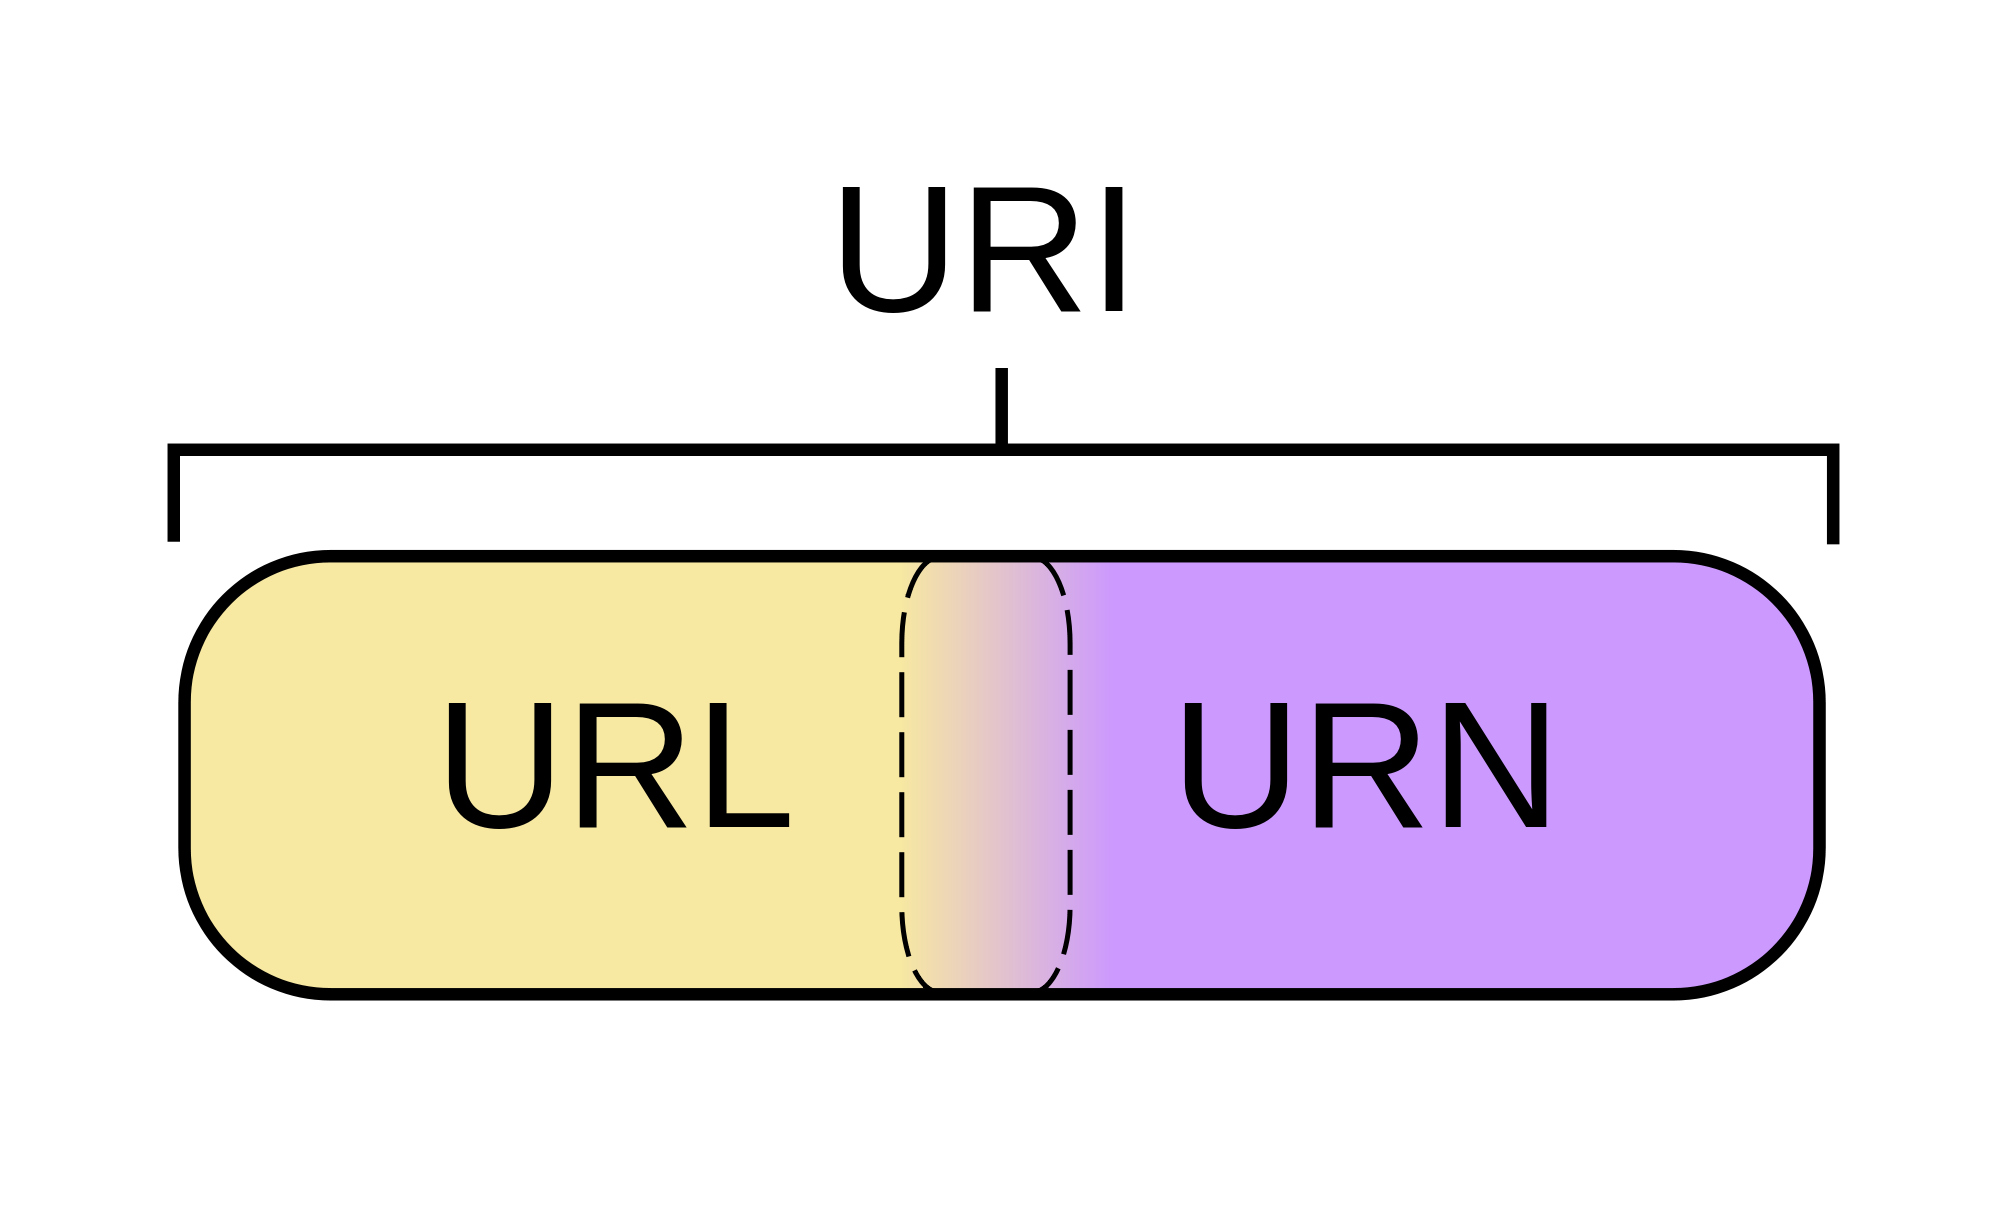
\includegraphics[width=0.4\textwidth]{resources/URI_Diagram}
    \caption{Diagramm zur Veranschaulichung der Teilmengenbeziehung zwischen den Adressierungsarten, Quelle \cite{wiki:urn}}
    \label{fig:uri_diagram}
\end{figure}